\section{Critique d'un protocole}

Pour vérifier la présence d'ions fer (III)  dans une solution, un élève propose le protocole sous la forme du schéma ci-dessous.


\begin{center}
	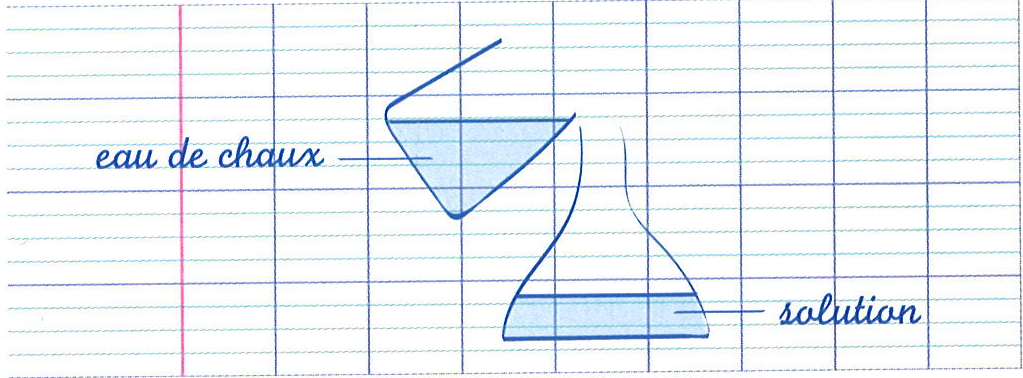
\includegraphics[scale=1]{img/proto}
\end{center}
\begin{questions}
	\question Rectifier l'erreur commise sur le réactif.
	\begin{solution}
		L'eau de chaux permet d'identifier le dioxyde de carbone. Pour identifier l'ion fer (III), il faut utiliser de la soude.
	\end{solution}
	
	\question Nommer le matériel utilisé.
	\begin{solution}
		Dans ce protocole, il utilise un bécher et un erlenmeyer.
	\end{solution}
	
	\question Quel matériel serait plus approprié ? Justifier.
	\begin{solution}
		Le test d'identification se fait avec une partie seulement de la solution à identifier et seules quelques goutes de réactif sont nécessaires. Il serait donc plus approprié de verser un peu de la solution dans un tube à essai et d'utiliser une pipette ou un compte goute pour le réactif.
	\end{solution}

\end{questions}